% !TEX TS-program = pdflatex
% !TEX encoding = UTF-8 Unicode

% TeX-M (r1.1)
% For my math classes at UT Austin
% Notes template created by Abdon Morales for the College of Natural Science
% and for the Department of Mathematics and Computer Science
% (c) 2019 - 2024 Abdon Morales and the University of Texas at Austin
% This is a notes template for a LaTeX document using the "article" class for Mathematics (Calculus)
% at the University of Texas at Austin.

% Last change made: Jan 27, 2024 1:40 AM CST

% See "book", "report", "letter" for other types of document.

\documentclass[11pt]{article} % use larger type; default would be 10pt

% Start of Article customization options and addons (for more help and information reference to Overleaf's guides and docs on Latex.
\usepackage[utf8]{inputenc} % set input encoding (not needed with XeLaTeX)

%%% Examples of Article customizations
% These packages are optional, depending whether you want the features they provide.
% See the LaTeX Companion or other references for full information.

%%% PAGE DIMENSIONS
\usepackage{geometry} % to change the page dimensions
\geometry{letterpaper} % or letterpaper (US) or a5paper or....
% \geometry{margin=2in} % for example, change the margins to 2 inches all round
% \geometry{landscape} % set up the page for landscape
%   read geometry.pdf for detailed page layout information

\usepackage{graphicx} % support the \includegraphics command and options
\usepackage{xcolor}

% \usepackage[parfill]{parskip} % Activate to begin paragraphs with an empty line rather than an indent

%%% PACKAGES
\usepackage{booktabs} % for much better looking tables
\usepackage{array} % for better arrays (eg matrices) in maths
\usepackage{paralist} % very flexible & customisable lists (eg. enumerate/itemize, etc.)
\usepackage{verbatim} % adds environment for commenting out blocks of text & for better verbatim
\usepackage{subfig} % make it possible to include more than one captioned figure/table in a single float
\usepackage{exercise}
% Math tools
\usepackage{mathtools}
\usepackage{amsmath}
\usepackage{tikz} % For charts, mathematical graphs, and etc
%% Equal symbol for L'Hospital Rule
\usepackage{tcolorbox}
\newcommand\LR{\stackrel{\mathclap{\normalfont\mbox{L.R}}}{=}}
% These packages are all incorporated in the memoir class to one degree or another...

%%% HEADERS & FOOTERS
\usepackage{fancyhdr} % This should be set AFTER setting up the page geometry
\pagestyle{fancy} % options: empty , plain , fancy
\renewcommand{\headrulewidth}{0pt} % customise the layout...
\lhead{}\chead{}\rhead{}
\lfoot{}\cfoot{\thepage}\rfoot{}

%%% SECTION TITLE APPEARANCE
\usepackage{sectsty}
\allsectionsfont{\sffamily\mdseries\upshape} % (See the fntguide.pdf for font help)
% (This matches ConTeXt defaults)

%%% ToC (table of contents) APPEARANCE
\usepackage[nottoc,notlof,notlot]{tocbibind} % Put the bibliography in the ToC
\usepackage[titles,subfigure]{tocloft} % Alter the style of the Table of Contents
\renewcommand{\cftsecfont}{\rmfamily\mdseries\upshape}
\renewcommand{\cftsecpagefont}{\rmfamily\mdseries\upshape} % No bold!
%%% END Article customizations

%%% The "real" document content comes below...

% Replace examples with the actual content you intend to put
\title{Monetary Policy \\ Introduction to Macroeconomics}
\author{Abdon Morales \\ The University of Texas at Austin \\ ECO 304L \\ Wayne Geerling}
\date{\today \\ Chapter 18 : Week 12}
%\date{} % Activate to display a given date or no date (if empty),
         % otherwise the current date is printed 
\begin{document}
\maketitle
At times, the U.S economy seems to hum along with unstoppable success; as a recent example, during the 26-year period from 1982 to 2007, there were just two recessions, and neither was severe or lengthy. During this period, many economists and other observers believed that the business cycle was essentially tamed once and for all. Some credit for this "great moderation" went to Alan Greenspan, the chairman of the board of governors of the Federal Reserve Board during much of this period. Analysts thought that his savvy handling of interest rates and money supply was the key to the sustained economic growth, and that enlightened supervision of central banks was the path to future economic growth throughout the world.

Unfortunately, the stability did not last; the Great Recession, which started in late 2007, plunged the United States into a deep economic downturn. Moreover, the slow recovery after 2009 seemed to underscore the limits of monetary policy during significant downturns, as the Fed's strategies to inject more money into the economy did not cure the problem as easily as some had forecast.

More recently, of course, after another long period of growth, the economy experienced a new shock driven by the spread of the COVID-19 virus. Once again, the Federal Reserve responded with aggressive action and a commitment to support the economy; the hope is that this move will avert a major, long-run recession, but it is clear that monetary policy cannot help us circumvent all downturns. In this chapter, we consider how changes in the money supply their way through the economy; we build on earlier material, drawing on what we learned about the loanable funds market and the aggregate demand-aggregate supply model. We begin by looking at the tools of monetary policy; we then examine how monetary policy affects the economy in the short run. We conclude the chapter by examining why monetary policy can't always turn an economy around.

\begin{tcolorbox}[width=\textwidth,colback={white},title={Big Questions},colbacktitle=yellow,coltitle=blue]
\begin{itemize}
\item What is the effect of monetary policy in the short run?
\begin{itemize}
\item In the short run, monetary policy can both speed up and slow down the economy.
\item Some prices are sticky in the short run; when some prices fail to adjust, changes in the money supply are essentially a change in real financial resources.
\item In the short run, expansionary monetary policy can stimulate the economy, increasing real GDP and reducing the unemployment rate.
\item In the short run, contractionary monetary policy can slow the economy, which may help to reduce inflation.
\end{itemize}
\item Why doesn't monetary policy always work?
\begin{itemize}
\item Monetary policy fails to produce real effects under three different circumstances. First, monetary policy has no real effect in the long run because all prices can adjust; second, if monetary policy is fully anticipated, prices adjust. Finally, if the economy is experiencing shifts in aggregate supply, monetary policy may be unable to restore normal growth, because monetary policy primarily through aggregate demand.
\end{itemize}
\item What is the Phillips curve?
\begin{itemize}
\item The Phillips curve is a theoretical negative relationship between inflation and unemployment rates; the modern consensus is that the Phillips curve is a short-run phenomenon that does not hold in the long-run.
\item The power of inflation to reduce unemployment is directly related to how people's inflation expectations adjust throughout the economy. Modern expectations theory allows for adjusting expectations, which is why most economists believe that the Phillips curve relationship does not hold in the long run.
\end{itemize}
\end{itemize}
\end{tcolorbox}
\section*{\textbf{What is the effect of monetary policy in the short run?}}
Across the globe, when economic growth stagnates and unemployment rises, we often look to the central bank to help the economy. Central banks in most countries use monetary policy to reduce interest rates and make it easier for people and businesses to borrow; this action generates new economic activity to get the economy moving again. In this chapter, we examine how monetary policy effects ripple through the economy.

We begin by considering the immediate, or short-run, effects. Recall the difference between the short run and the long run in macroeconomics. The \textit{long run} is a period of time long enough for all prices to adjust, but in the \textit{short run}, some prices - often the prices of resources such as wages for workers and interest rates for loans - are inflexible.
\subsection*{An overview of monetary policy in the short run}
Monetary policy affects your actions, and your actions affect the macroeconomy; investment increases because you spend on equipment, inventory, and a physical location. Investment is part of aggregate demand, so aggregate demand increase; as a result of the increase, in aggregate demand, real GDP increases and unemployment falls as your output rises and you hire workers. This is what monetary policy can do in the short run: it expands the amount of credit (loanable funds) available and paves the way for economic expansion.

Now let's trace the impact of this kind of monetary policy on the entire macroeconomy. In doing so, we draw heavily on what we have presented in preceding chapters; here, pulled together from previous chapters is a short list of concepts we will use (the chapters are identified so you can review as necessary):
\begin{enumerate}
\item The Fed uses the interest on reserve balances (IORB) to implement monetary policy. When the IORB falls, banks have an incentive to loan out their reserves, and this then multiplies the money supply and reduces other interest rates (Chapter 17).
\item Lower interest rates increase the quantity of investment demand, just as lower prices increase the quantity demanded in any product market (Chapter 9).
\item Investment is one component of aggregate demand, so changes in investment indicate corresponding changes in aggregate demand (Chapter 13)
\item In the short run, increases in aggregate demand increase output and lower unemployment rate (Chapter 13).
\end{enumerate}

We have studied each of these concepts separately; now it is time to put them together for a complete picture of how monetary policy works.
\subsection*{Expansionary Monetary Policy}
There are two types of monetary policy: expansionary and contractionary; \textbf{\textcolor{red}{Expansionary monetary policy}} occurs when a central bank acts to increase the money supply in an effort to stimulate the economy. Traditionally, the Fed expanded the money supply through open-market purchases.

Recently, expansionary monetary policy has shifted to lowering the interest on reserve balances (IORB), incentivizing banks to increase lending, which increases the money supply and reduces the interest rates.

\begin{center}
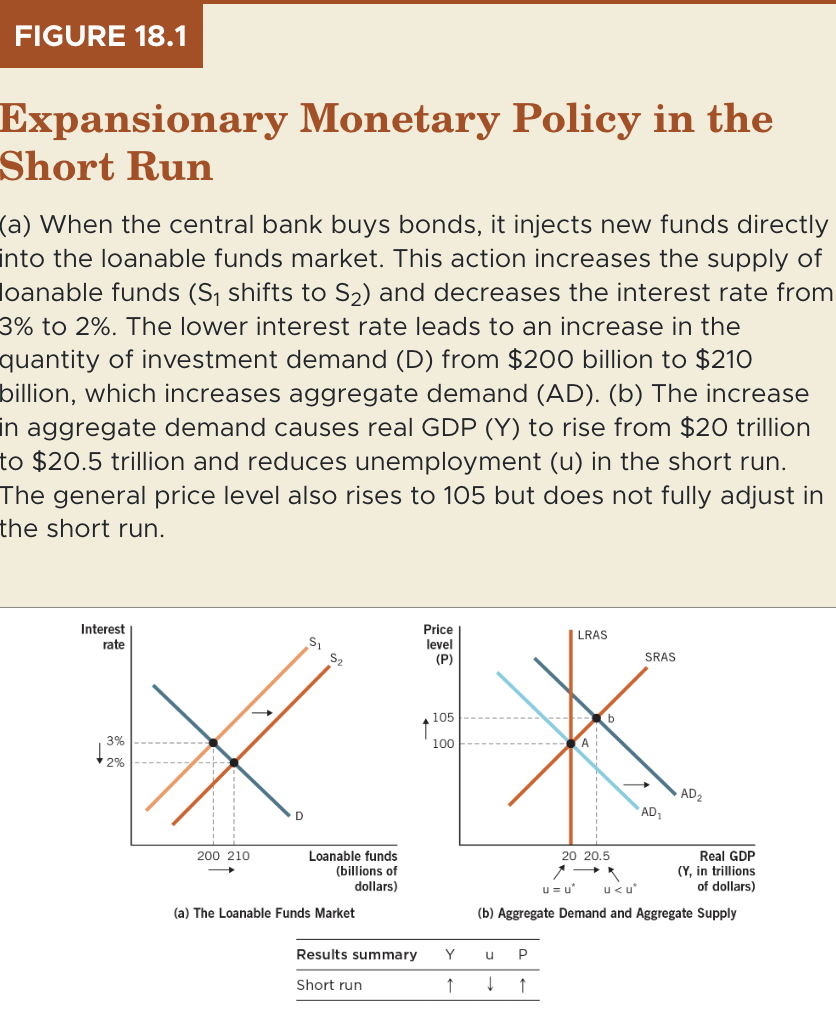
\includegraphics[scale=0.5]{images/Figure 18.1.png} 
\end{center}
Because investment is a component of aggregate demand, an increase in the quantity of investment demand also increases aggregate demand, as pictured in panel (b) of Figure 18.1. Remember from Chapter 13 that aggregate demand derives from four sources: C, I, G, and NX; when investment (I) increases, aggregate demand increases from $\text{AD}_1$ to $\text{AD}_2$.

In the short run, increases in aggregate demand lead to increases in real GDP; in panel (b) of Figure 18.1, the economy moves from an initial long-run equilibrium at point A to a short-run equilibrium at point B. Real GDP increases from \$20 trillion to \$20.5 trillion; the increase in GDP leads to more jobs through the increase in aggregate demand; therefore, it also leads to lower unemployment. Finally, the general price level rises from 100 to 105; this price level increase in only partial. In the short run, output prices are more flexible than input prices, which are sticky and do not adjust.

In summary, in the short run, expansionary monetary policy reduces unemployment (u) and increases real GDP (Y). In addition, the overall price level (P) rises somewhat as flexible prices increase in the short run. These results are summarized in the table at the bottom of Figure 18.1
\subsubsection*{\textcolor{olive}{Real versus Nominal effects}}
\subparagraph*{
We have seen that changes in the quantity of money lead to real changes in the economy. You may wonder: if a central bank can create jobs and real GDP by simply increasing the money supply, why would it ever stop? After all, fiat money is just paper! The answer is that while there is a short-run incentive to increase the money supply, these effects wear off in the long run, as prices adjust and then drive down the value of money.
}
\begin{center}
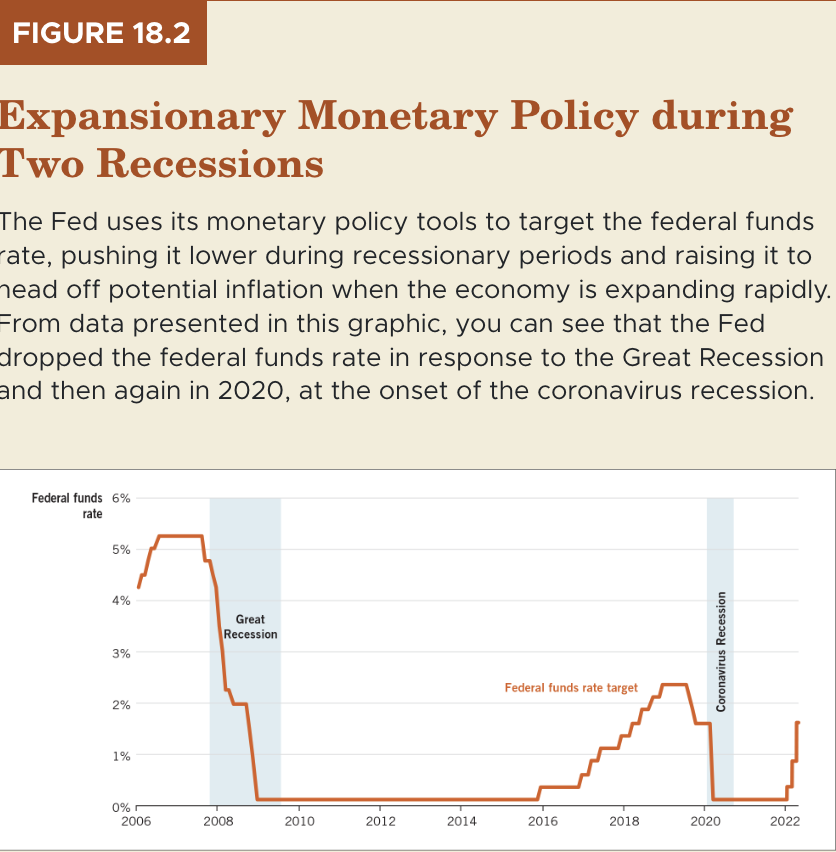
\includegraphics[scale=0.5]{images/Figure 18.2.png} 
\end{center}
\subparagraph*{The new money devalues the entire money supply, because prices rise; but because college students get the money first, you get it before any prices adjust. So these new funds represent an increase in real purchasing power for you. This is why monetary policy can have an immediate, real short-run effects: initially, no prices have adjusted, but as prices adjust in the long run, the effects of the new money wear off.}
\subparagraph*{Injecting new money into the economy eventually causes inflation, but inflation doesn't happen right away, and prices does not rise uniformly. During the time that prices are increasing, the value of money is constantly moving downward. Figure 18.3 illustrates the real purchasing power of money as time goes by. Panel (a) shows adjustment to the price level; when new money enters the economy (at time $t_0$), the price level begins to rise in the short run and then reaches its new level in the long run (at time $t_{\text{LR}}$. Panel (b) shows the value of a dollar relative to these price-level adjustments; when the new money enters the economy, each dollar has its highest value, because prices have not yet adjusted. In the short run, as prices rise, the real purchasing power of each dollar gradually falls; in the long run, all prices adjust, and the real value of each dollar reaches its lower level. At this point, the real effects of the monetary policy dissipate completely.}

\begin{center}
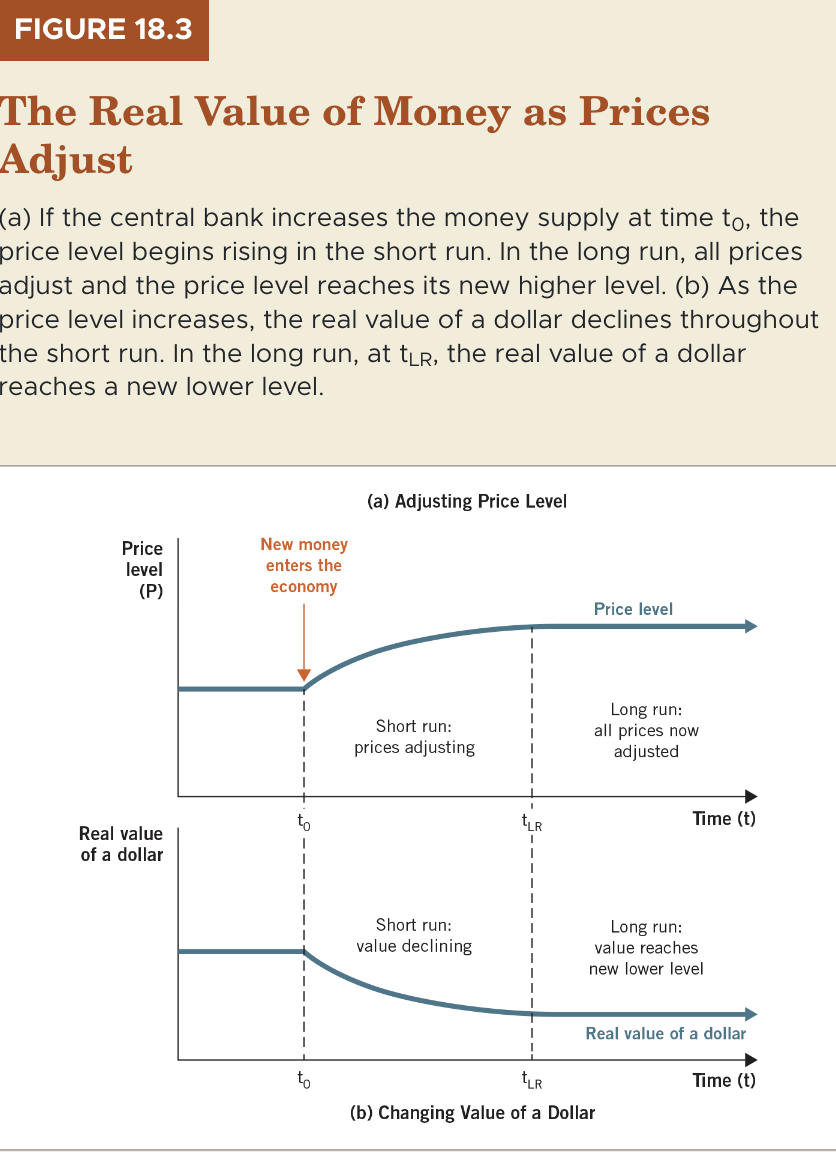
\includegraphics[scale=0.5]{images/Figure 18.3.png} 
\end{center}
\subsubsection*{\textcolor{olive}{Unexpected inflation hurts some people}}
\subparagraph*{Let's now consider how expansionary monetary policy affects different people across the economy. The basic macroeconomic results, summarized in Figure 18.1, seem very positive: real GDP goes up, the unemployment rate falls, and there is some inflation. Consider that you are living in an economy where these conditions exist. Everywhere you look, the news seems positive, as the media, politicians, and firms focus on the expanding economy; but this action does not help everybody.}
\subparagraph*{Monetary policy derives its potency from sticky prices, but if your price (or wage) is stuck, inflation hurts you.}
\subparagraph*{Inflation harms input suppliers that have sticky prices; in addition to workers, lenders (the suppliers to funds used for expansion) are another prominent group harmed when inflation is greater than anticipated.}
Later in this chapter, we talk about incentives for these resource suppliers to correctly anticipate inflation. For now, we just note that unexpected inflation, while potentially, helpful to the overall economy, is harmful to those who adjust slowly.
\subsection*{Contractionary Monetary Policy}
We have seen how the central bank uses expansionary monetary policy to stimulate the economy. However, sometimes policymakers want to slow the economy; \textbf{\textcolor{red}{contractionary monetary policy}} occurs when a central bank takes action that reduces the money supply in the economy is expanding rapidly and the central bank fears inflation.

To implement contractionary monetary policy, the Fed can increase the IORB or sell bonds in the loanable funds market. Either way, the interest rate in the loanable funds market rises as supply declines.

\begin{center}
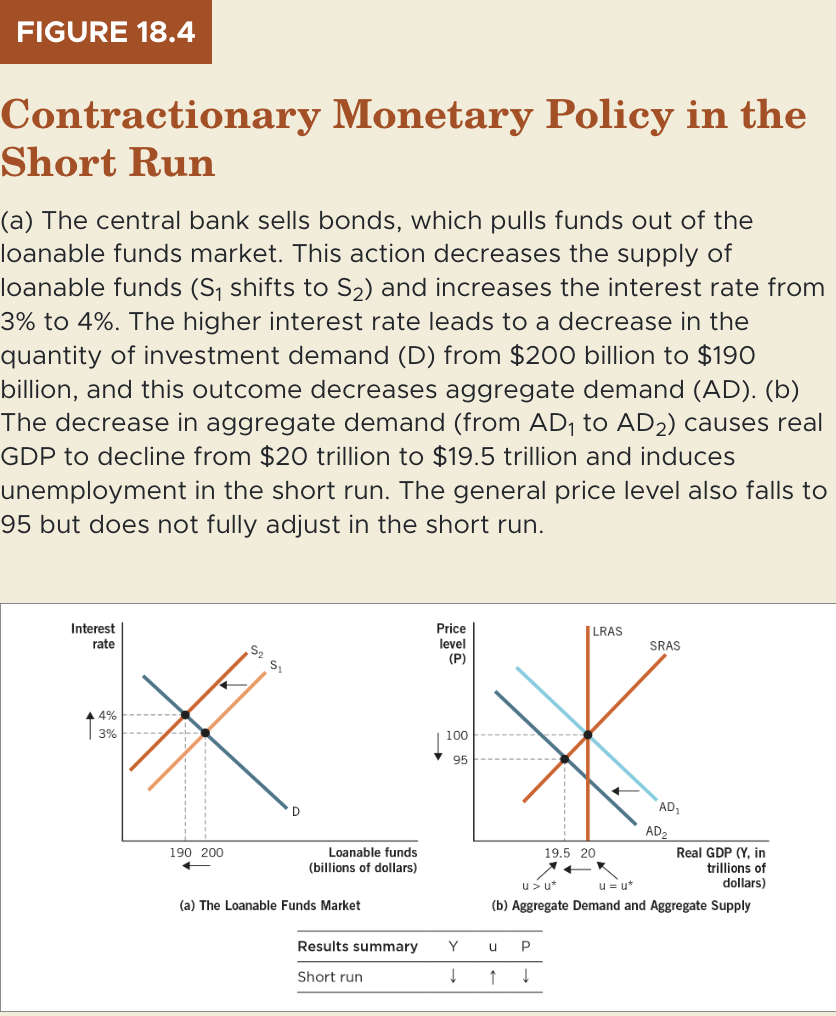
\includegraphics[scale=0.5]{images/Figure 18.4.png} 
\end{center}
These short-run results are again the result of fixed resource prices for the firm. A lower money supply leads to downward pressure on prices (P), but sticky resource prices mean that firms cannot adjust their workers' wages or the terms of their loans in the short run. Therefore, firms reduce output and lay off some workers. This is why we see real GDP (Y) falling and the unemployment rate (u) rising. These results are summarized in the table at the bottom of the figure.

\begin{center}
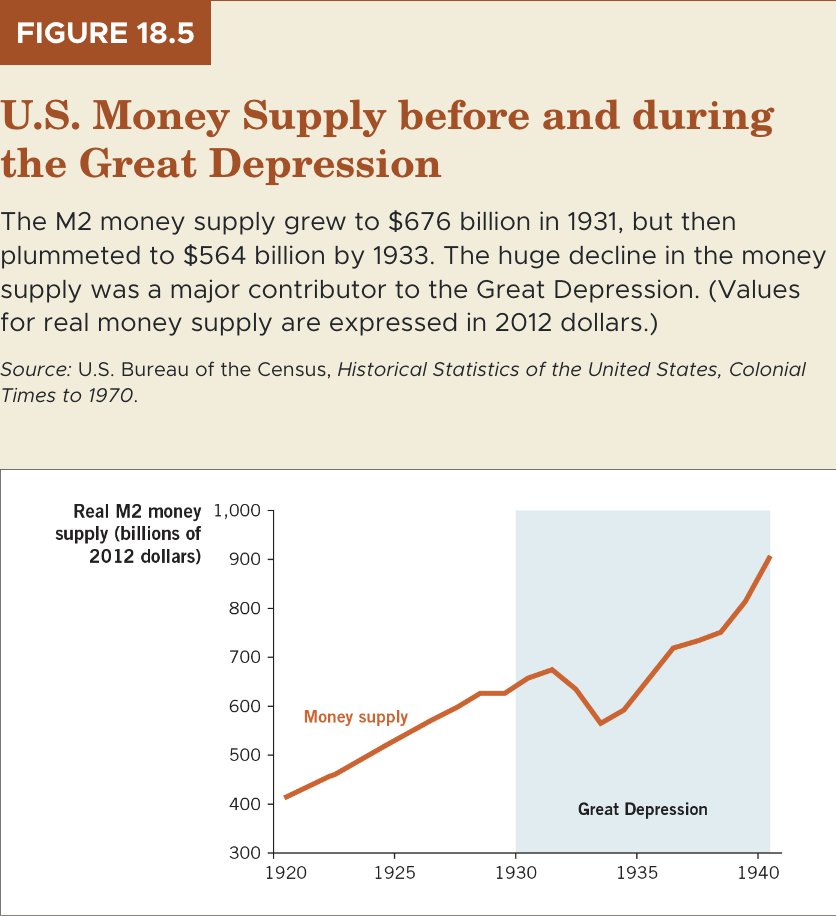
\includegraphics[scale=0.5]{images/Figure 18.5.png} 
\end{center}

\section*{\textbf{Why doesn't monetary policy always work?}}
So far, we have seen that monetary policy can have real effects on the macroeconomy. By shifting aggregate demand, monetary policy can affect real GDP, unemployment, and the price level; but most economists feel that monetary policy is limited in what it can accomplish. In this section, we consider these three limitations: first, we look at the diminished effects of monetary policy in the long run; next, we consider how expectations can dampen the effects of monetary policy. Finally, we examine the limitations of monetary policy when economic downturns are caused by shifts in aggregate supply rather than aggregate demand.

\subsection*{Long-run adjustment}
We have noted that some prices taken longer to adjust than others and that the long run is a period long enough for \textit{all} prices to adjust. Output prices can adjust relatively quickly; in contrast, input prices, such as workers' wages, are often the slowest prices to adjust. After all, wages are sometimes set by contracts; moreover, money illusions (see Chapter 8) can make input suppliers reluctant to lower their prices. But in the long run is a period sufficient for all prices to change, even wage contracts, which eventually expire.

Both types of prices affect the decisions made at firms across the economy, and therefore both affect output and unemployment.

% Might need some more notes here

\begin{center}
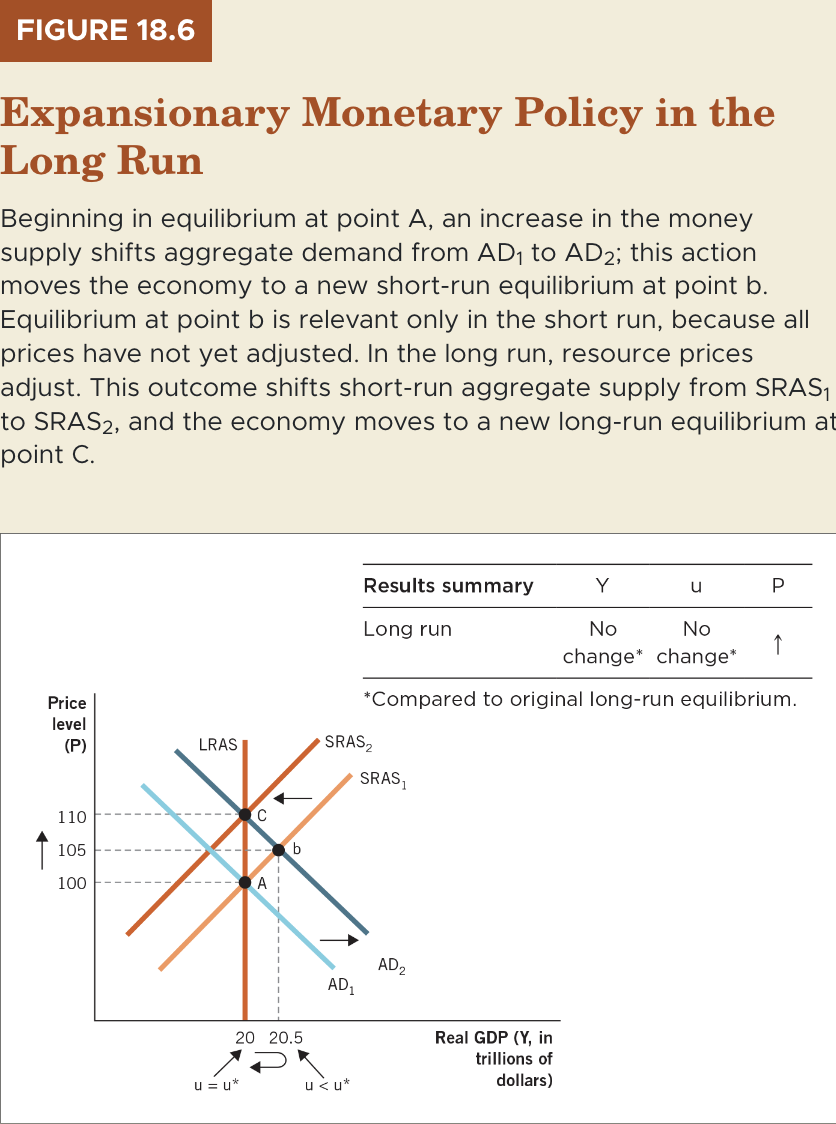
\includegraphics[scale=0.5]{images/Figure 18.6.png} 
\end{center}
One important implication of these long-run results is the lack of real economic effects from monetary policy; in the long run, all prices adjust. Therefore, in the long run, monetary policy does not affect real GDP or unemployment; the only predictable result of more money in the economy over the long run is inflation. As we discussed in Chapter 8, the cause of inflation is monetary growth; you now can understand why, in the context of the aggregate demand-aggregate supply model.

From one perspective, our long-run results may seem strange: central banks can't do much in the long run to affect the real economy. However, this statement might also seem logical, since it's possible to increase the money supply by just printing more paper money; but printing more paper money doesn't affect the economy's long-run productivity or its ability to produce. These outcomes are determined by resources, technology, and institutions; the idea that the money supply does not affect real economic variables is known as \textbf{\textcolor{red}{monetary neutrality}}.

Given that money is neutral in the long run, why do the Federal Reserve and other central banks employ short-run monetary policy? In fact, many of the substantive debates in macroeconomics focus on the relative importance of the short versus long run. Some economists believe it is best to focus on short-run effects, which are very real; after all, during recessions people often lose their jobs, which can be a very painful experience. When the money supply expands, firms can borrow more cheaply and hire more workers; from this perspective, central banks ought to take a very active role in the macroeconomy by increasing the money supply during economic downturn and contracting the money supply during economic expansions. This policy can then potentially smooth out the business cycle.

Other economists discount the short-run expansionary effects of monetary policy and instead focus on the problems of inflation. In Chapter 8, we explored the negative effects of inflation; these include price confusion, wealth redistribution, and uncertainty about future price levels. These by-products of inflation can stifle economic growth.

In the next section, we consider the potency of monetary policy when market participants expect inflation ahead of time.

\subsection*{Adjustments in expectations}
Unexpected inflation harms workers and other resource suppliers who have fixed prices in the short run. Therefore, workers normally expect a certain level of inflation and expect to see it reflected by annual pay adjustments or in contractual cost-of-living adjustments that are sometimes tied to inflation rates. The key incentive for anticipating the correct rate of inflation is straightforward: surprise inflation harms people, but when inflation is expected, the real effects on the economy are limited.

Let's look at inflation expectations in the context of the aggregate demand-aggregate supply model. Figure 18.7 shows how monetary expansion affects aggregate demand and aggregate supply when it is expected. Expansionary monetary policy shifts aggregate demand from $\text{AD}_1$ to $\text{AD}_2$, but if this effect is expected, short-run aggregate supply shifts to the left from $\text{SRAS}_1$ to $\text{SRAS}_2$.

In Chapter 13, we discussed how short-run aggregate supply shifts back when workers and resource suppliers expect higher future prices, because they do not want their real prices to fall. If short-run aggregate supply shifts along with the shift in aggregate demand, the economy goes immediately to equilibrium at point C. Therefore, monetary policy has no real effect on the economy - real GDP and unemployment do not change; the only lasting change is nominal, because the price level rises from 100 to 110. Monetary policy has real effects only when some prices are sticky; but if inflation is expected, prices are not sticky since they adjust because people plan on the inflation. To the extent that all prices rise, the effect of monetary policy is limited, even in the short run.

\begin{center}
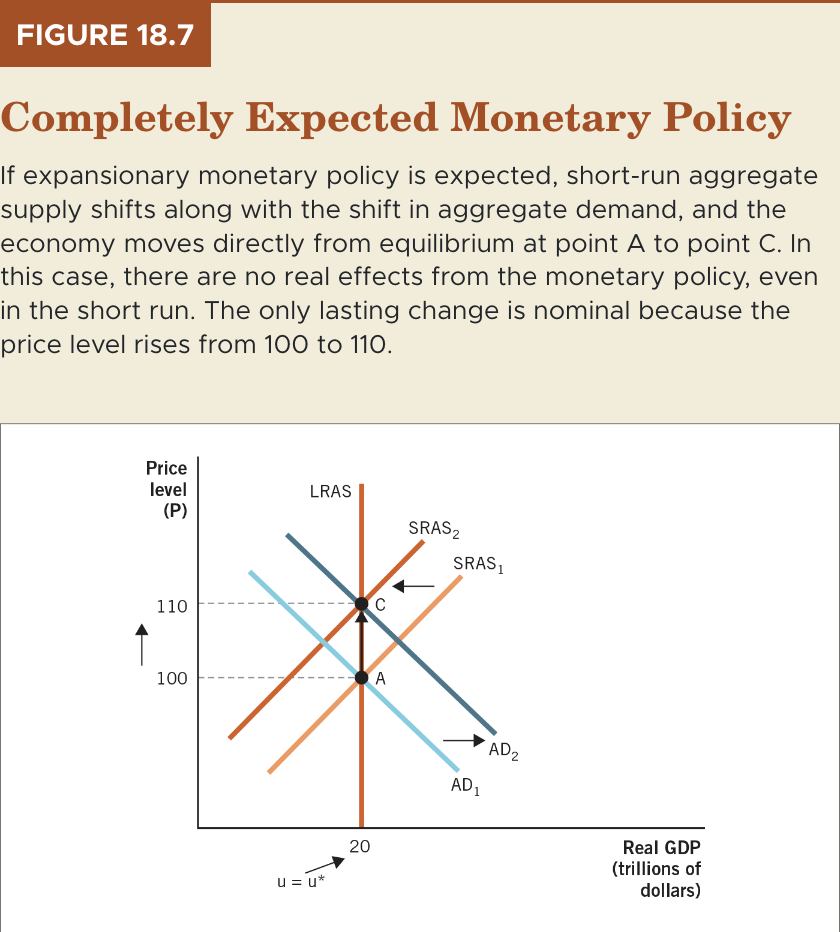
\includegraphics[scale=0.5]{images/Figure 18.7.png} 
\end{center}

\subsection*{Aggregate supply shifts and the Great Recession}
We have seen that monetary supply affects the economy by shifting aggregate demand; thus, if a recession results from reduced aggregate demand, monetary policy can stabilize the economy and return it to higher levels of real GDP and lower unemployment, but not all downturns are a result of aggregate demand shifts. Declines in aggregate supply can also lead to recession; and when supply shifts cause the downturn, monetary policy is less likely to restore the economy to its pre-recession conditions.

The Great Recession that began in 2007 seems to have included both shifts of aggregate supply and shifts of aggregate demand. In Chapter 14, we argued that the widespread problems in financial markets at that time negatively affected key institutions in the macroeconomy. Further, new financial regulations restricted banks' ability to lend at levels equal to those in effect prior to 2008; the result was a shift backward in long-run aggregate supply. In addition, as people's real wealth and expected future income levels declined, aggregate demand shifted to the left.

\begin{center}
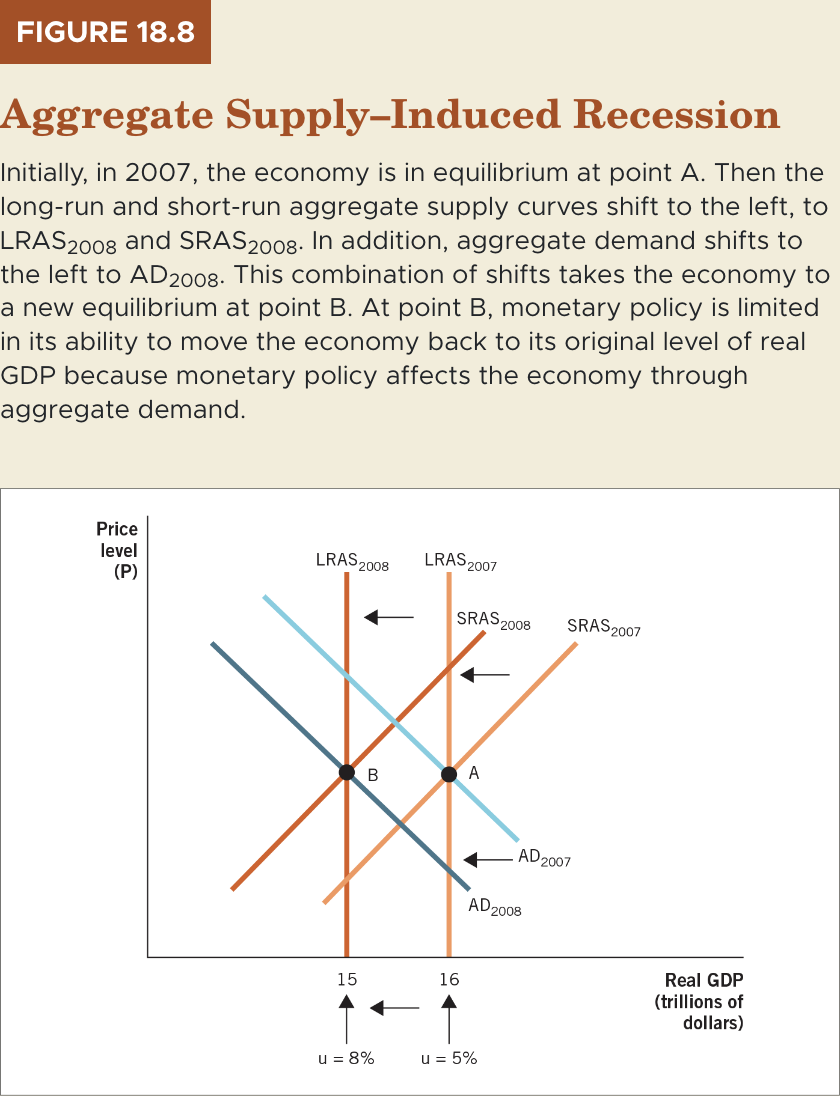
\includegraphics[scale=0.5]{images/Figure 18.8.png} 
\end{center}

The dilemma is that at point B, monetary policy is limited in its ability to permanently move output back to its prior level. Even if monetary policy shifts aggregate demand back to $\text{AD}_{2007}$, this shift is not enough to eliminate the recession. Furthermore, as we have stressed throughout this chapter, the effects of monetary policy wear off in the long run.

Thus, in the wake of the Great Recession, the U.S economy continued to struggle with slow growth and high unemployment, even after significant monetary policy interventions. The bottom line is that monetary policy does not enable us to avoid or fix every economic downturn.
\section*{\textbf{What is the Phillips Curve?}}
We have seen that monetary policy can stimulate the economy in the short run. Increasing the money supply increases aggregate demand, which can lead to higher real GDP, lower unemployment, and a higher price level (inflation). The relationship between inflation and unemployment is of particular interest to economists and noneconomists alike; it is at the heart of the debate regarding the power of monetary policy to affect the economy. In this section, we examine this relationship by looking at the Phillips curve.

\subsection*{The traditional short-run Phillips curve}
In 1958, British economist A.W Phillips noted a negative relationship between wage inflation and unemployment rates in the United Kingdom. Soon thereafter, U.S economists Paul Samuelson and Robert Solow extended the analysis to inflation and unemployment rates in the United States; this short-run negative relationship between inflation and unemployment rates became known as the \textbf{\textcolor{red}{Phillips curve}}. Before looking at Phillips curve data, let's consider the theory behind the Phillips curve in the context of the aggregate demand-aggregate supply model.

\begin{center}
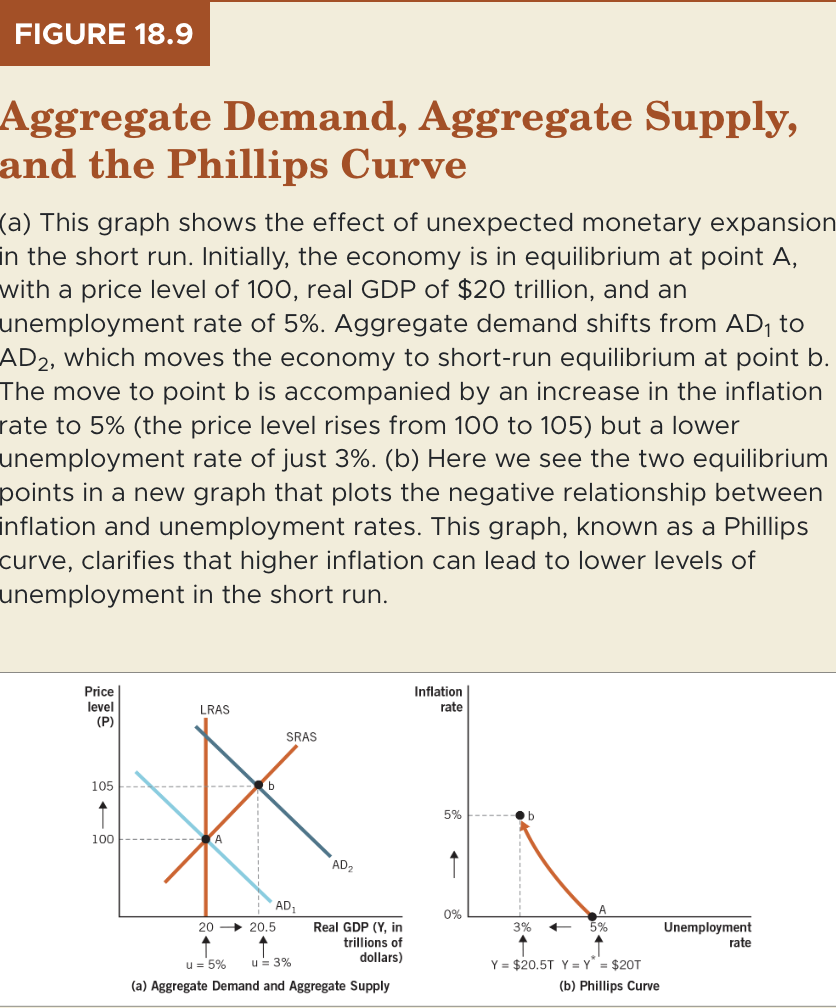
\includegraphics[scale=0.5]{images/Figure 18.9.png}\\
\textit{Panel (a) of Figure 18.9 shows how unexpected monetary expansion affects the economy in the short run.}
\end{center}
This is the theory behind the Phillips curve relationship: monetary expansion stimulates the economy and brings some inflation, and this outcome reduces the unemployment rate. Similarly, lower inflation is associated with higher unemployment rates; this negative relationship between inflation and unemployment is captured in panel (b) of Figure 18.9, which graphs a Phillips curve.

This negative relationship between inflation and unemployment rates is consistent with Phillips' observations and also with what Samuelson and Solow saw when they plotted historical data. Figure 18.10 plots U.S inflation and unemployment rates from 1948 to 1969, which includes the period just before and just after the work of Samuelson and Solow. The numerical values plotted represent the years; it's not hard to visualize a Phillips curve relationship in this data: most years with high inflation rates had low unemployment rates, while most years with low inflation rates had high unemployment rates.
\begin{center}
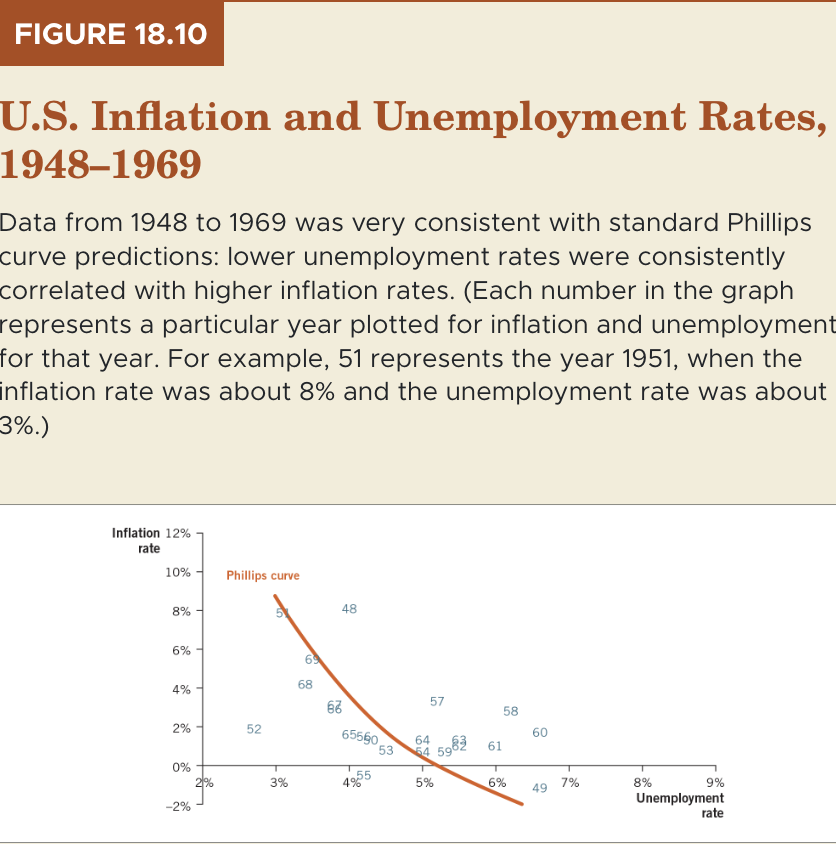
\includegraphics[scale=0.5]{images/Figure 18.10.png}
\end{center}
The Phillips curve implies a powerful role for monetary policy. It implies that a central bank choose higher or lower unemployment rates simply by adjusting the rate of inflation in an economy. If this is a realistic observation, a central bank can always steer an economy out of recession, simply by creating inflation.

But we have already seen that monetary policy does not always have real effects on the economy. Next we consider the long run, when the real effects of monetary policy wear off. After that, we look at how expectations also mitigate the effects of monetary policy.

\subsection*{The Long-Run Phillips Curve}
When all prices are free to adjust, there are no real effects from monetary policy; that is, there are no effects on real GDP or unemployment. Therefore, the long-run Phillips curve looks different from the standard, short-run Phillips curve. Figure 18.11 shows both short-run and long-run Phillips curves; initially, at point A, there is no inflation in the economy and the unemployment rate is 5\%. Then monetary expansions increases the inflation rate to 5\%, and the unemployment rate falls to 3\% in the short run. This short-run equilibrium is indicated as point b, but when prices adjust in the long run, the unemployment rate returns to 5\% and the economy moves to a new equilibrium at point C. Inflation is the only result of monetary expansion in the long run.
\begin{center}
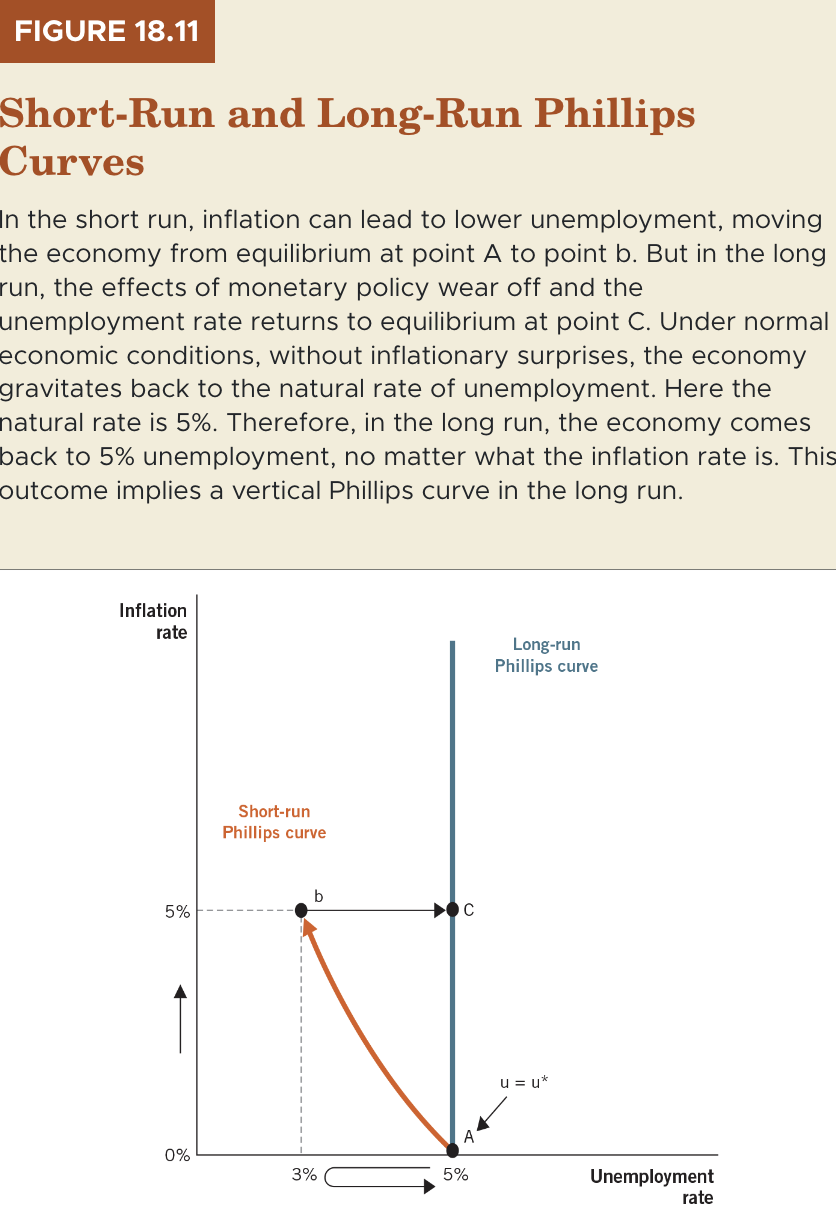
\includegraphics[scale=0.5]{images/Figure 18.11.png} 
\end{center}
In Figure 18.11, the unemployment rate is equal to the natural rate (5\%) before inflation, and in the long run it returns to the natural rate. Thus, under normal economic conditions including a scenario with no surprise inflation; we expect the unemployment rate to equal to the natural rate ($u = u$*). Monetary policy can push the unemployment rate down, but only in the short run.

We have also learned that the effects of inflation are dampened or eliminated when inflation is fully expected. We saw this earlier in the context of the aggregate demand-aggregate supply model; now look more closely at inflation expectations and how they affect the Phillips curve relationship.

\subsection*{Expectations and the Phillips Curve}
We have seen that expected inflation has no real effects on the macroeconomy, even in the short run, because when inflation is expected, all prices adjust. To explore this further, we consider alternative theories of how people form expectations. This topic may seem like one for microeconomics or perhaps even psychology, but it is particularly relevant to monetary policy because the effects of expected inflation are completely different from the effects of unexpected inflation. When inflation is expected, long-term contracts can reflect inflation and mitigate its effect; but when inflation is unexpected, wages and other prices don't adjust immediately, and the result is economic expansion.

\subsubsection*{\textbf{\textit{Adaptive expectation theory}}}
\subparagraph*{
In the late 1960s, economists Milton Friedman and Edmund Phelps hypothesized that people adapt their inflation expectations to their prior experience. The contributions of Friedman and Phelps came to be known as adaptive expectations; \textbf{\textcolor{red}{Adaptive expectation theory}} hold that people's expectations of future inflation are based on their most recent experience. 
}
\begin{center}
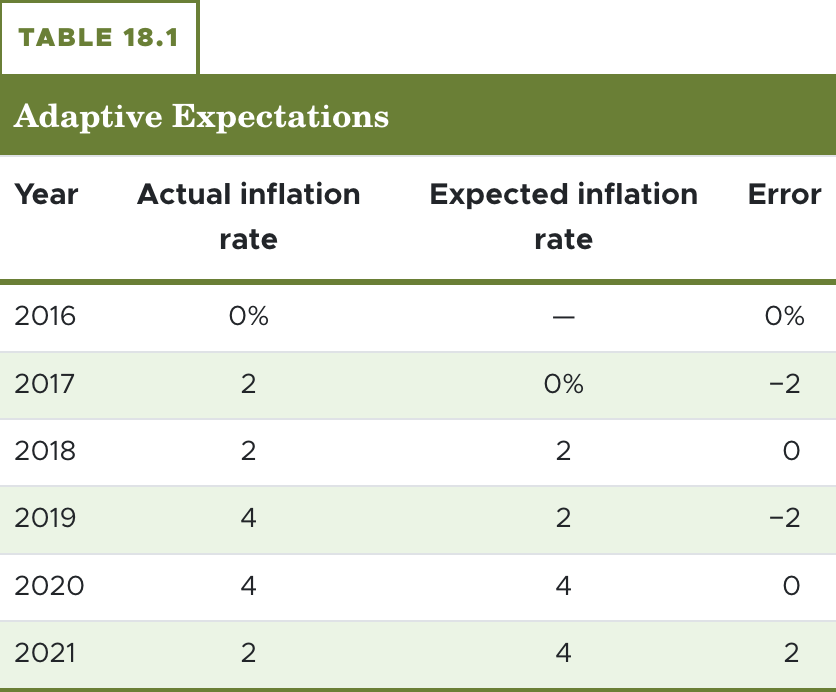
\includegraphics[scale=0.5]{images/Table 18.1.png} 
\end{center}
\subparagraph*{
When the inflation rate \textit{accelerates}, however, people do underestimate inflation. Note that it is also possible under adaptive expectations theory to overestimate inflation. Note that it is also possible under adaptive expectations theory to overestimate inflation; overestimation happens when inflation rates fall.
}
\subparagraph*{
The idea behind adaptive expectations theory is not overly complex, but it revolutionized the way economists think about monetary policy. If expectations adapt, then monetary policy may not have real effects, even in the short run. Expansionary monetary policy can stimulate the economy and reduce unemployment, but only if it is unexpected.}
\subparagraph*{This was the insight of Friedman and Phelps; their basic reasoning was that people are not quite as simpleminded as the basic Phillips curve implies. Given that surprise inflation harms people, they have an incentive to anticipate inflation and, at the very least, learn from past experience. And yet, the data from the 1960s, shown in Figure 18.10, were certainly consistent with the traditional Phillips curve. But Friedman and Phelps challenged the accepted wisdom in 1968 and predicted that the Phillips curve relationship would not last. In particular, they predicted that high inflation would not always deliver low unemployment - a prediction that proved correct.}
\subparagraph*{Figure 18.12 shows U.S unemployment and inflation rates for the period 1948 to 1979, with data for the 1970s presented in orange. (As in Figure 18.10, the numerical value represents the year) Clearly, the 1970s were a difficult decade for the macroeconomy; the prior Phillips curve relationship fell apart - compare Figure 18.12 with Figure 18.10. In the 1970s, inflation was high, and so was unemployment; these macroeconomic conditions are now known as \textbf{\textcolor{red}{stagflation}}, which is the combination of high unemployment and high inflation. The stagflation of the 1970s baffled many economists who believed in the validity of the Phillips curve.}

\subsubsection*{\textcolor{olive}{Rational expectations theory}}
\subparagraph*{
Expectations theory evolved yet again in the 1970s and 1980s, in part because of disenchantment with certain implications of adaptive expectations. Expectations are seemingly always a step behind reality; and these errors are predictable. 
}
\subparagraph*{\textbf{\textcolor{red}{Rational expectations theory}} holds that people form expectations on the basis of all available information. If people form expectations rationally, they use more than just today's current level of inflation to predict next year's. Rational expectations are different from adaptive expectations consider only past experience.}
\begin{center}
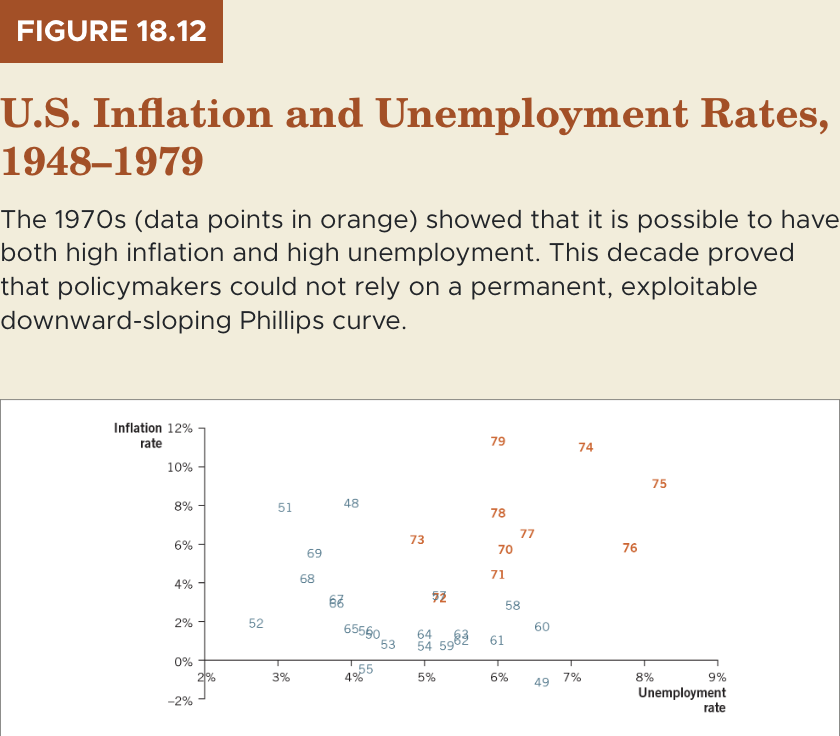
\includegraphics[scale=0.5]{images/Figure 18.12.png} 
\end{center}
\subparagraph*{Rational expectations theory does not imply that people always predict inflation correctly. No one knows exactly what the level of inflation will be next year; prediction errors are inevitable. But people are unlikely to underpredict consistently, even when inflation is accelerating. Rational expectations theory identifies prediction errors as random, like the flip of a coin - sometimes positive and sometimes negative.}

\subsection*{A modern view of the Phillips curve}
The short-run Phillips curve built on the assumption that inflation never adjust, but economists today recognize that the harmful effects of inflation provide an incentive to predict the future inflation. Therefore, not all inflation is surprise inflation, and when inflation is not a surprise, it does not affect the unemployment rate. So we need to reconsider how different expectations affect the Phillips curve relationship.

\begin{center}
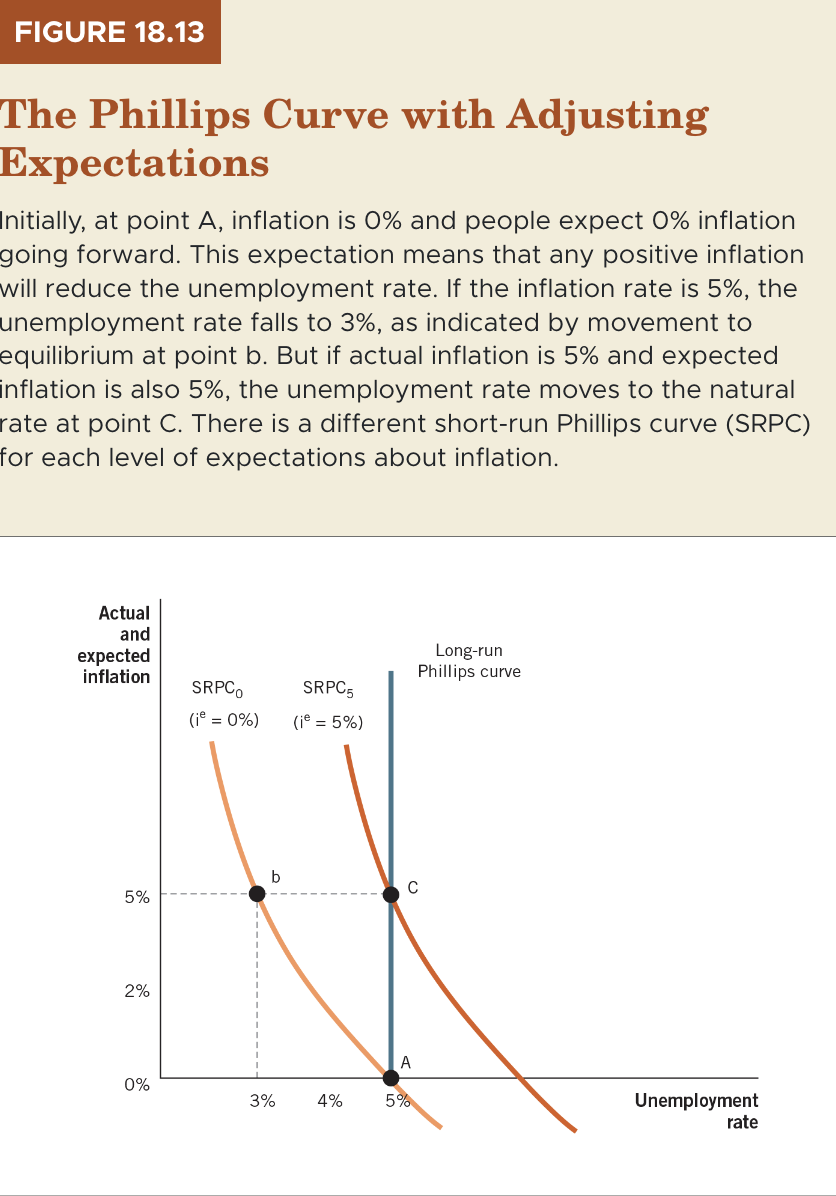
\includegraphics[scale=0.5]{images/Figure 18.13.png} 
\end{center}
\begin{center}
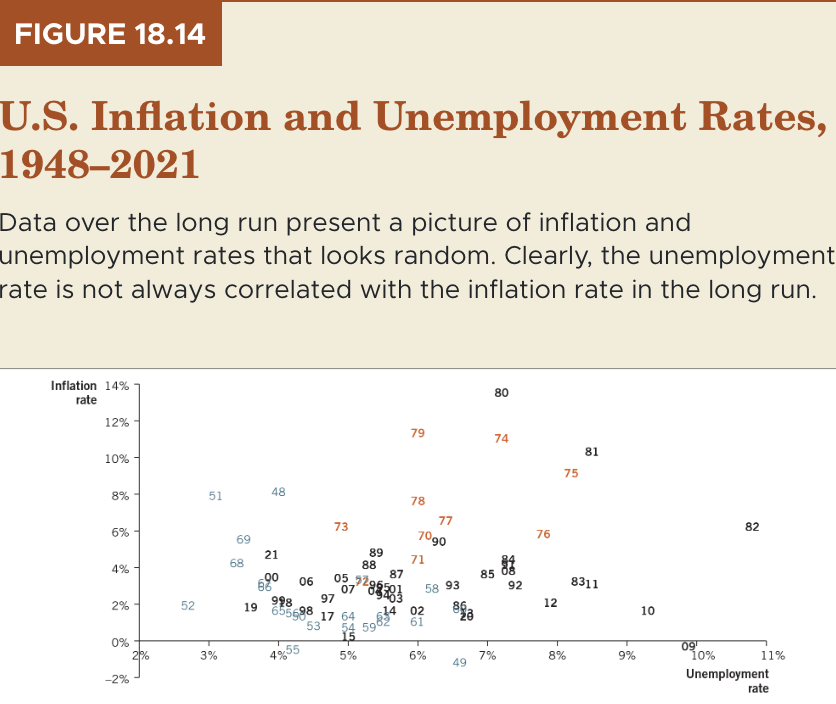
\includegraphics[scale=0.5]{images/Figure 18.14.png}\\
\textit{Figure 18.14 shows unemployment and inflation data from 1948 through 2021}
\end{center}
From this complete data set, it seems clear that there is no long-run stable relationship between inflation and unemployment. In fact, the data appear to be randomly distributed; economists today believe that there are many factors that influence the unemployment rate in the economy, and inflation rate is just one factor.

\subsection*{Implication for Monetary Policy}
We can now use what we've learned about expectations theory and the Phillips curve to evaluate monetary policy recommendations. \textbf{\textcolor{red}{Active monetary policy}} involves the strategic use of monetary policy to counteract macroeconomic expansions and contractions; in the 1960s, before the development of expectations theory, monetary policy prescriptions were strictly activist: increase inflation during economic downturns, and reduce inflation when the economy is booming. This policy assumed that the Phillips curve relationship between inflation and unemployment would hold up in the long run.

Modern expectations theory prescribes greater caution; if people anticipate the strategies of the central bank, the power of the monetary policy erodes. If expectations adjust, the optimal monetary policy is to maintain transparency and stability; this conclusion holds if expectations are formed either adaptively or rationally.

Many economists feel that monetary policy surprise actions should be minimized; \textbf{\textcolor{red}{passive monetary policy}} occurs when central banks purposefully choose only to stabilize the money supply and price levels through monetary policy. In particular, passive policy does not seek to use inflation to affect real variables, including unemployment and real GDP. In the United States, the Federal Reserve has moved markedly in this direction since the early 1980s (Ronald Reagan); Ben Bernanke, Janet Yellen, Jerome Powell, and other chairs of the Federal Reserve Board have consistently taken actions that lead to fewer surprises in monetary policy.

\section*{\textbf{Conclusion}}
We began this chapter with the observation that central banks can't always control the macroeconomy; if they could, the U.S economy certainly would not have experienced the sustained downturn that began at the end of 2007. So what can a central bank do? In the short run, if monetary policy is a surprise, a central bank can stimulate the economy and perhaps lessen the effects of a recession; but these results are mitigated when people come to anticipate monetary policy actions.

In the next two chapters, we turn to the international facets of macroeconomics; international trade, exchange rates, and international finance are becoming more important as the world economy becomes more integrated.
\end{document}